\documentclass[11pt,a4paper]{article}

\usepackage[a4paper,margin=1in]{geometry}
\usepackage{titlesec}
\usepackage{hyperref}
\usepackage{enumitem}
\usepackage{listings}
\usepackage{xcolor}
\usepackage{parskip}
\usepackage{graphicx}
\usepackage{booktabs}
\usepackage{amsmath}
\usepackage{tikz}
\usepackage{caption}
\usepackage{float}

\setlength{\parindent}{0pt}

\definecolor{lightgray}{gray}{0.95}
\definecolor{codecolor}{rgb}{0.1,0.1,0.4}

\lstset{
  backgroundcolor=\color{lightgray},
  basicstyle=\ttfamily\small,
  breaklines=true,
  frame=single,
  showstringspaces=false,
  columns=fullflexible,
  keywordstyle=\color{codecolor}\bfseries,
  commentstyle=\color{gray}\itshape
}

\titleformat{\section}{\Large\bfseries}{\thesection}{1em}{}
\titleformat{\subsection}{\large\bfseries}{\thesubsection}{1em}{}
\titleformat{\subsubsection}{\normalsize\bfseries}{\thesubsubsection}{1em}{}

\title{\textbf{MICS Open Network Security}\\[0.5em]
\large Background: DNS Covert Channels}

\begin{document}
\maketitle

\begin{abstract}
This document introduces DNS covert channels: techniques that abuse the Domain Name System (DNS) to hide, tunnel, or exfiltrate data. Before explaining the attack techniques and examples, we introduce the different concepts necessary for the attack to work as well as the attack itself.
\end{abstract}


\section{Motivation \& threat overview}
A DNS attack is an exploit where a malicious actor takes advantage of vulnerabilities in the Domain Name System (DNS) to disrupt services, redirect users to malicious websites, or gain unauthorized access to an organization's resources. 

This lab will focus on covert channels, a technique used to establish a secret, unauthorized communication link between a compromised system inside a network and an attacker's external server. Attackers exploit the fact that DNS traffic is generally trusted and rarely inspected closely by firewalls and other security measures to hide their malicious activities.

\section{DNS (Domain Name System)}
\subsection{What is DNS?}
DNS, or Domain Name System, is the Internet's phone book that translates human-friendly domain names like \texttt{www.google.com} into machine-readable IP addresses (e.g., 172.217.160.142). This allows users to visit websites by typing an easy-to-remember name instead of a long string of numbers, which computers use to locate and connect to each other on a network. 

There are four DNS components involved in resolving a domain name when loading a web page:
\begin{itemize}[noitemsep]
  \item \textbf{Root servers:} The root servers are the first step, and the most authoritative, in translating (resolving) human-readable host names into IP addresses. They can be thought of as the library that knows the names of every rack of dictionaries (the top-level delegations).
  \item \textbf{TLD name servers:} The top-level domain (TLD) servers can be thought of as a specific rack of dictionaries for a TLD (for example, \texttt{.com}). A TLD nameserver is the next step in the search for a specific IP address and knows the authoritative nameservers for second-level domains.
  \item \textbf{Authoritative servers:} The authoritative nameserver holds the actual records for a domain (for example, \texttt{example.com}) and is responsible for returning the requested IP address or other resource record.
  \item \textbf{Resolver:} The resolver acts like a librarian who is asked to find the translation in a particular book somewhere in the library. A recursive resolver queries the hierarchy on behalf of the client and returns the final answer.
\end{itemize}

Below is a representation of the DNS hierarchy:

\begin{figure}[H]
    \centering
    \includegraphics[width=0.8\linewidth]{images/hierarchy.png}
    \caption{DNS hierarchy}
    \label{fig:hierarchy}
\end{figure}

\subsection{Typical DNS message flow}
A simplified recursive lookup:
\begin{enumerate}[noitemsep]
  \item The client asks its stub resolver (often the OS or local resolver) for \texttt{host.example.com}.
  \item If the resolver does not have the answer, it queries root servers, then TLD servers, then the authoritative server for \texttt{example.com}.
  \item The authoritative server responds with the requested record(s).
\end{enumerate}

\begin{figure}[H]
    \centering
    \includegraphics[width=1\linewidth]{images/trace.png}
    \caption{DNS resolver route}
    \label{fig:placeholder}
\end{figure}


\subsection{Common DNS record types}
DNS records are the entries inside the ``dictionary.'' They record different types of information used by different services:
\begin{itemize}[noitemsep]
  \item \textbf{A} IPv4 address
  \item \textbf{AAAA} IPv6 address
  \item \textbf{NS} Name server delegation
  \item \textbf{MX} Mail exchange
  \item \textbf{TXT} Arbitrary text (commonly abused for data)
  \item \textbf{CNAME} Canonical name (alias)
\end{itemize}


\section{DHCP (Dynamic Host Configuration Protocol)}
\subsection{What is DHCP?}
DHCP automates network configuration of hosts/client. It makes the network aware of a new host and gives the host the configuration needed to communicate: assigning IP addresses, default gateway, DNS servers, and other options.

\subsection{Typical DHCP flow}
\begin{enumerate}[noitemsep]
  \item \textbf{DHCPDISCOVER}: Client broadcasts to find DHCP servers.
  \item \textbf{DHCPOFFER}: Server offers a lease with an IP address and options.
  \item \textbf{DHCPREQUEST}: Client requests the offered lease.
  \item \textbf{DHCPACK}: Server acknowledges and finalizes the lease.
\end{enumerate}


\section{Covert Channels vs. Tunneling in DNS}

While both covert channels and tunneling exploit DNS traffic to carry hidden information, they differ in purpose, design, and scale. Understanding this distinction is critical when analyzing DNS-based communication in security monitoring.

\subsection{Conceptual Difference}

A covert channel hides small amounts of information inside legitimate DNS behavior. It typically modifies or encodes data in protocol fields (such as transaction IDs, flags, or subdomain case) so that the message blends into normal traffic. The goal is stealth, not speed. Covert channels are often used for command-and-control signals or for exfiltrating limited data without detection.

A DNS tunnel, on the other hand, establishes a full communication pathway through DNS by encapsulating arbitrary data, such as TCP or HTTP packets inside DNS queries and responses. It allows an external client and server to exchange continuous data even when other protocols are blocked. The goal here is connectivity, not subtlety.

\subsection{Operational Characteristics}

\begin{table}[h!]
\centering
\begin{tabular}{|p{3cm}|p{5cm}|p{5cm}|}
\hline
\textbf{Feature} & \textbf{Covert Channel} & \textbf{DNS Tunneling} \\
\hline
Purpose & Hidden signaling or low-rate data leakage & Full bidirectional data transfer over DNS \\
\hline
Data Volume & Very low (bits or bytes per query) & High (can carry full sessions) \\
\hline
Structure & Encodes bits within header fields, flags, or label case & Encapsulates entire payloads inside DNS records (A, TXT, NULL) \\
\hline
Stealth & High - mimics legitimate DNS behavior & Lower - large, repetitive, or high-entropy subdomains are easier to detect \\
\hline
Throughput & Extremely limited & Moderate, limited by query rate and resolver latency \\
\hline
Use Cases & C2 signaling, status beacons, small data exfiltration & Bypassing firewalls, remote shell access, VPN-like tunnels \\
\hline
\end{tabular}
\end{table}

\subsection{Why the Difference Matters}

From a defender’s perspective, the two mechanisms require distinct detection approaches:

\begin{itemize}
    \item \textbf{Covert channels} demand fine-grained behavioral analysis, looking for subtle anomalies such as flag patterns, transaction-ID sequences, or case variations.
    \item \textbf{Tunnels} produce statistical anomalies: high query rates, long encoded subdomains, frequent TXT responses, or persistent communication with a single external domain.
\end{itemize}

Recognizing whether traffic represents tunneling or covert signaling guides both mitigation strategy and forensic interpretation. Tunnels indicate an active data pipeline, while covert channels suggest stealthy control or leakage within otherwise normal traffic.

In short, covert channels hide within DNS, whereas tunneling uses DNS as the channel itself. The difference lies in intent and scale: covert communication seeks invisibility; tunneling seeks reachability.



\section{DNS Covert Channel Techniques}
\label{channels}

\subsection{DNS Packet Structure and Exploitable Fields}

Understanding DNS packet structure reveals which fields can be exploited for covert channels. Figure \ref{fig:dns-packet} shows the layout of a DNS packet with exploitable fields highlighted in red.

\begin{figure}[h!]
\centering
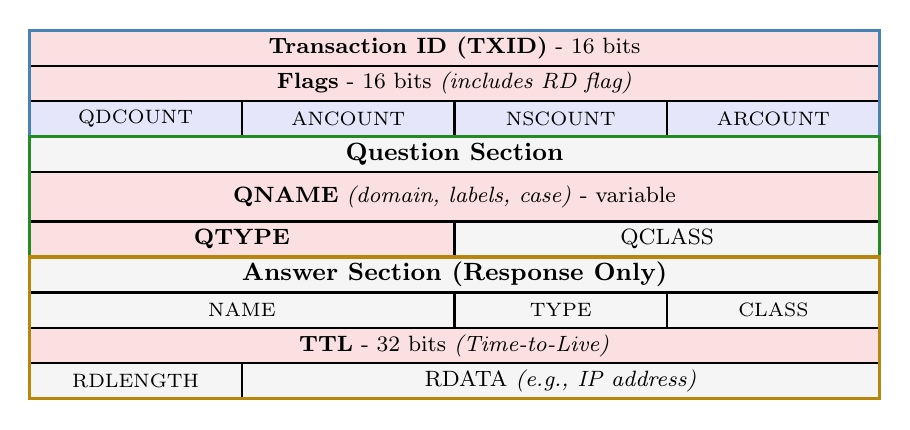
\begin{tikzpicture}[scale=0.9, every node/.style={font=\footnotesize}]
    % Define colors
    \definecolor{exploitable}{RGB}{220,50,50}
    \definecolor{headercolor}{RGB}{230,230,250}
    \definecolor{sectioncolor}{RGB}{245,245,245}
    \definecolor{headeroutline}{RGB}{70,130,180}
    \definecolor{questionoutline}{RGB}{34,139,34}
    \definecolor{answeroutline}{RGB}{184,134,11}

    % Header fields - exploitable ones with red background
    \draw[thick, fill=exploitable!15] (0,0) rectangle (12,0.5);
    \node at (6,0.25) {\textbf{Transaction ID (TXID)} - 16 bits};

    \draw[thick, fill=exploitable!15] (0,-0.5) rectangle (12,0);
    \node at (6,-0.25) {\textbf{Flags} - 16 bits \textit{(includes RD flag)}};

    % Non-exploitable header fields - 4 across
    \draw[thick, fill=headercolor] (0,-1) rectangle (3,-0.5);
    \node at (1.5,-0.75) {\scriptsize QDCOUNT};
    \draw[thick, fill=headercolor] (3,-1) rectangle (6,-0.5);
    \node at (4.5,-0.75) {\scriptsize ANCOUNT};
    \draw[thick, fill=headercolor] (6,-1) rectangle (9,-0.5);
    \node at (7.5,-0.75) {\scriptsize NSCOUNT};
    \draw[thick, fill=headercolor] (9,-1) rectangle (12,-0.5);
    \node at (10.5,-0.75) {\scriptsize ARCOUNT};

    % Header Section outline
    \draw[very thick, headeroutline] (0,0.5) rectangle (12,-1);

    % Question Section header
    \draw[thick, fill=sectioncolor] (0,-1.5) rectangle (12,-1);
    \node at (6,-1.25) {\textbf{\small Question Section}};

    % Question fields - exploitable
    \draw[thick, fill=exploitable!15] (0,-2.2) rectangle (12,-1.5);
    \node at (6,-1.85) {\textbf{QNAME} \textit{(domain, labels, case)} - variable};

    \draw[thick, fill=exploitable!15] (0,-2.7) rectangle (6,-2.2);
    \node at (3,-2.45) {\textbf{QTYPE}};
    \draw[thick, fill=sectioncolor] (6,-2.7) rectangle (12,-2.2);
    \node at (9,-2.45) {QCLASS};

    % Question Section outline
    \draw[very thick, questionoutline] (0,-1) rectangle (12,-2.7);

    % Answer Section header
    \draw[thick, fill=sectioncolor] (0,-3.2) rectangle (12,-2.7);
    \node at (6,-2.95) {\textbf{\small Answer Section (Response Only)}};

    % Answer fields - compact layout
    \draw[thick, fill=sectioncolor] (0,-3.7) rectangle (6,-3.2);
    \node at (3,-3.45) {\scriptsize NAME};
    \draw[thick, fill=sectioncolor] (6,-3.7) rectangle (9,-3.2);
    \node at (7.5,-3.45) {\scriptsize TYPE};
    \draw[thick, fill=sectioncolor] (9,-3.7) rectangle (12,-3.2);
    \node at (10.5,-3.45) {\scriptsize CLASS};

    % TTL - exploitable
    \draw[thick, fill=exploitable!15] (0,-4.2) rectangle (12,-3.7);
    \node at (6,-3.95) {\textbf{TTL} - 32 bits \textit{(Time-to-Live)}};

    \draw[thick, fill=sectioncolor] (0,-4.7) rectangle (3,-4.2);
    \node at (1.5,-4.45) {\scriptsize RDLENGTH};
    \draw[thick, fill=sectioncolor] (3,-4.7) rectangle (12,-4.2);
    \node at (7.5,-4.45) {RDATA \textit{(e.g., IP address)}};

    % Answer Section outline
    \draw[very thick, answeroutline] (0,-2.7) rectangle (12,-4.7);
\end{tikzpicture}
\caption{DNS packet structure with exploitable fields highlighted. Red-shaded fields can be manipulated to encode covert data: Transaction ID, Flags (RD bit), QNAME (subdomain, labels, case), QTYPE, and TTL (in responses). Colored outlines distinguish the three main sections: blue for Header, green for Question, and gold for Answer. More channels can be built using other header fields, but these are the ones tackled in this lab.}
\label{fig:dns-packet}
\end{figure}

\subsection{Single-Packet Subdomain Encoding Channels}

The most straightforward covert channel approach embeds entire messages within a single DNS query's subdomain label. These high-throughput channels can transmit substantial data in few queries but create distinctive patterns that make them easier to detect.

\subsubsection{Base32 Encoding}

Base32 encoding uses a 32-character alphabet (A-Z and 2-7) to represent binary data, with each character encoding 5 bits since $2^5=32$. The encoding process converts a message to binary, splits it into 5-bit chunks, maps each chunk to a Base32 character, and uses the resulting string as a subdomain. For example, the message ``Hello'' becomes \texttt{jbswy3dp.example.com}. This encoding is DNS-safe because it uses only case-insensitive alphanumeric characters that are valid in domain names.

The efficiency is approximately 1.6 characters per byte, which means a 63-character DNS label can hold roughly 39 bytes of raw data. Security analysts looking for Base32-encoded channels should watch for high-entropy subdomains that contain only lowercase letters a-z and digits 2-7, notably lacking 0, 1, 8, and 9. The random appearance of these subdomains - strings like ``jbswy3dpeblw64tmmq'' - stands out sharply against typical human-readable domain names.

\subsubsection{Hexadecimal Encoding}

Hexadecimal encoding represents each byte as two hex digits (0-9, a-f), making it simpler but less efficient than Base32. At 2 characters per byte, a 63-character label holds approximately 31 bytes of raw data. The encoding is straightforward: convert each byte to its two-digit hex representation and concatenate the results.

Detection signatures include subdomains containing only hexadecimal characters with no letters beyond 'f', even-length strings (since each byte becomes exactly two characters), and high entropy. For instance, ``4869'' encoding ``Hi'' looks suspicious compared to legitimate subdomain patterns. The absence of letters g through z is a particularly strong indicator of hex encoding.

\subsubsection{XOR + Base32 Encryption}

Adding a layer of security, this channel applies XOR encryption with a secret key before Base32 encoding. The XOR operation combines each byte of the message with corresponding bytes of the key (repeating the key cyclically if needed), producing encrypted bytes that are then Base32-encoded. This provides confidentiality - without the correct key, decoded data appears as random garbage rather than readable text.

The efficiency remains identical to plain Base32 at 5 bits per character, and importantly, the encrypted channel is indistinguishable from regular Base32 encoding when observed on the network. Defenders cannot determine whether high-entropy Base32 subdomains are encrypted or simply encoded without attempting decryption. However, XOR encryption remains vulnerable to known-plaintext attacks and frequency analysis, making it suitable for obfuscation rather than strong cryptographic protection.

\subsection{Multi-Packet Header and Structure-Based Channels}

Rather than embedding large amounts of data in subdomain labels, these channels manipulate DNS header fields or structural elements across multiple queries. They sacrifice throughput dramatically but gain significantly better stealth since the manipulated fields vary naturally in legitimate DNS traffic.

\subsubsection{RD Flag (Recursion Desired) Channel}

The RD flag covert channel exploits a single bit in the DNS header that normally indicates whether the client wants recursive resolution. By toggling this flag between queries, an attacker can encode one bit per query: RD flag set represents binary 1, RD flag clear represents binary 0. To transmit a message, the attacker converts it to binary and sends each bit as a separate DNS query with the appropriate RD flag value.

This channel's bandwidth is minimal - just 1 bit per query, requiring 8 queries to transmit a single byte. Encoding the letter ``A'' (0x41 = binary 01000001) requires 8 queries with RD flag values: clear, set, clear, clear, clear, clear, clear, set. A 100-byte message would need 800 separate queries. Despite this inefficiency, the channel offers exceptional stealth because RD flag variation is completely normal in real networks. Some clients request recursion while others don't, making this pattern blend seamlessly with legitimate traffic. The flag is also preserved reliably by recursive resolvers, unlike some header fields that may be modified in transit. However, when many queries are performed in rapid sequence from a single host, the stealth advantage diminishes significantly - maintaining true stealth requires very low throughput, effectively limiting the channel's practical utility.

\subsubsection{TXID (Transaction ID) Channel}

The Transaction ID channel encodes data directly in the 16-bit TXID field that normally matches queries to responses. The attacker splits a message into 2-byte chunks and uses each chunk's numeric value as a transaction ID. For example, the message ``Hi'' has hex value 0x4869, which equals 18537 in decimal - this becomes the TXID for a single query. At 16 bits (2 bytes) per query, this channel operates 16 times faster than the RD flag method.

However, reliability is a significant concern. Many recursive DNS resolvers override transaction IDs for security reasons to prevent TXID collision attacks, and NAT devices may modify them as well. This makes the TXID channel most effective when querying authoritative DNS servers directly rather than through recursive resolvers. The stealth level is moderate: while varying TXIDs appear natural, security tools analyzing the semantic meaning of TXID sequences (such as whether they decode to ASCII text) can detect suspicious patterns.

\subsubsection{DNS TTL Channel}

The DNS TTL channel operates differently from most covert channels because it encodes data in DNS responses rather than queries. An attacker controlling an authoritative DNS server can set the TTL field of resource records to encode bytes of data. Each response's TTL value maps to one byte of the message, providing a bandwidth of 1 byte per query-response pair.

A critical distinction must be made between DNS TTL and IP TTL, as these are fundamentally different fields that are often confused. IP TTL is a network-layer field in the IP packet header that decrements at each router hop, making it unsuitable for covert channels since its value changes unpredictably during transmission. DNS TTL, in contrast, is an application-layer field measured in seconds that indicates how long a DNS record should be cached. This value remains constant during transit, making it reliable for encoding. Furthermore, DNS TTL only appears in DNS responses (not queries), while IP TTL appears in every IP packet. The reliability and constant nature of DNS TTL makes it superior for covert channel applications compared to the unreliable, decrementing IP TTL.

\subsubsection{Query Type (QTYPE) Channel}

The QTYPE channel varies the DNS query type field to encode data. By mapping different data values to different query types - for instance, A=0, AAAA=1, MX=2, TXT=3, CNAME=4, NS=5, and so on - an attacker can encode several bits per query. With 8 to 16 commonly used query types that won't appear too suspicious, this provides roughly 3 to 4 bits per query.

The stealth level is moderate because varying query types does occur naturally when applications look up different kinds of DNS records. However, unusual sequences or patterns, such as rapidly cycling through all possible query types repeatedly, would appear suspicious to behavioral analysis systems.

\subsubsection{Label Count Channel}

The label count channel encodes data by varying the number of subdomain labels (the depth of the domain hierarchy). If an attacker uses $n$ different possible label counts, each query can encode $\log_2(n)$ bits. DNS technically allows up to 127 labels, which would provide a theoretical capacity of $\log_2(127) \approx 6.99$ bits per query - nearly a full byte. For example, one label like \texttt{example.com} might represent 0, while seven labels like \texttt{a.b.c.d.e.f.g.example.com} represents 6.

In practice, using extreme label depths would be highly suspicious, so attackers typically limit themselves to 8-16 different depths, encoding 3-4 bits per query while maintaining better stealth. The variation in subdomain depth does occur naturally, but highly regular patterns or extreme depths quickly trigger anomaly detection systems.

\subsubsection{Case Toggle Channel}

The case toggle channel exploits an interesting property of DNS: the protocol is case-insensitive according to RFC specifications, yet the original case of characters is preserved in queries and observable on the network. By varying the case of characters in a domain label, an attacker can encode bits with lowercase representing 0 and uppercase representing 1. This provides approximately 1 bit per alphabetic character, or roughly 1 byte per 8-character label.

The stealth level is exceptionally high because DNS servers treat the queries identically regardless of case, and case variation in domain names appears completely natural. The channel works reliably through all DNS infrastructure since case preservation is standard behavior. While case-based encoding is a well-documented covert channel technique in security literature, many legacy and commercial DNS security systems prioritize detecting high-volume anomalies and entropy-based patterns over subtle per-character case variations, making this channel difficult to detect without specialized monitoring.

\subsection{Multi-Channel Combination}

Advanced adversaries sometimes combine multiple covert channels within single DNS queries to maximize data throughput. For example, a query might simultaneously use case toggling in the subdomain label, vary the label count, set a specific TXID value, and manipulate the RD flag. When these channels operate independently on separate fields or aspects of the query, the total information capacity equals the sum of individual channel capacities. For instance, if case toggling encodes 8 bits in the subdomain characters, label count encodes 3 bits, TXID encodes 16 bits, and RD flag encodes 1 bit, a single query can theoretically carry 28 bits total. This additive property holds because each encoding mechanism uses a distinct, non-overlapping portion of the DNS packet structure.

However, this approach significantly increases detection risk. Each channel creates its own anomalies - high entropy, unusual patterns, suspicious header values - and when combined, these anomalies compound and become more likely to trigger security alerts. The implementation complexity also increases substantially, as the attacker must carefully coordinate multiple encoding schemes and decode them correctly on the receiving end. Most real-world attacks prefer simpler approaches with adequate bandwidth over complex multi-channel schemes.

\subsection{Channel Comparison and Trade-offs}

\begin{table}[h]
\centering
\small
\begin{tabular}{@{}lllll@{}}
\toprule
\textbf{Channel} & \textbf{Bits/Query} & \textbf{Stealth} & \textbf{Direction} & \textbf{Reliability} \\
\midrule
Base32 & ~312 (39 bytes) & Low & Request & High \\
Hex & ~248 (31 bytes) & Low & Request & High \\
XOR+Base32 & ~312 (39 bytes) & Medium & Request & High \\
RD Flag & 1 & Very High & Request & High \\
TXID & 16 & Medium & Request & Medium \\
DNS TTL & 8 & High & Response & High \\
QTYPE & 3-4 & Medium & Request & High \\
Label Count & 3-7 & Medium & Request & High \\
Case Toggle & ~8 & Very High & Request & High \\
\bottomrule
\end{tabular}
\caption{DNS covert channel characteristics}
\end{table}

To illustrate the dramatic differences in throughput, consider exfiltrating a 100-byte document using different channels: Base32 requires only 3 queries, hexadecimal needs 4 queries, but RD flag demands 800 queries, TXID needs 50 queries, and label count (at 3 bits per query) requires 267 queries.

The fundamental trade-off in covert channel design balances throughput against stealth. High-throughput channels like Base32 and hexadecimal encoding are efficient, transmitting substantial data quickly, but they create obvious anomalies in the form of high-entropy, random-looking subdomains that stand out dramatically in traffic analysis. Low-throughput channels like RD flag and case toggle are painfully slow but blend naturally with legitimate DNS traffic patterns. Attackers must choose their approach based on operational needs: quickly exfiltrating large volumes of data versus maintaining a stealthy command-and-control channel over extended periods.

\section{Detection, Prevention, and Monitoring}

Defending against DNS covert channels requires multiple overlapping layers of detection, prevention, and monitoring. No single technique provides complete protection; effective defense demands a comprehensive approach combining statistical analysis, behavioral monitoring, network controls, and incident response capabilities.

\subsection{Detection Techniques}

\subsubsection{Statistical Anomaly Detection}

Statistical analysis forms the foundation of covert channel detection by identifying traffic that deviates from normal baseline behavior. Subdomain entropy analysis measures the randomness of domain labels using Shannon entropy. Normal human-readable domains like ``google'' or ``amazon'' typically score below 3.0 bits per character, while encoded data approaches 4.5-5.0 bits per character. This sharp difference makes entropy a powerful initial filter.

The query uniqueness ratio examines what fraction of queries from a host are for unique, never-before-seen subdomains. Calculated as $\frac{\text{Unique Subdomains}}{\text{Total Queries}}$, normal traffic typically shows ratios below 0.3 because caching causes repeated queries for the same domains. Covert channels, however, often exceed 0.9 uniqueness since each query encodes different data. Label length distribution analysis reveals whether subdomains consistently use maximum allowed lengths (63 characters) or show unusual patterns, both indicators of encoding.

Character frequency analysis detects encoding schemes by their characteristic patterns. Base32-encoded domains contain only lowercase a-z and digits 2-7, completely lacking 0, 1, 8, and 9. Hexadecimal encoding uses only 0-9 and a-f, with no letters beyond f. Normal domains favor vowels and common consonants.

Temporal pattern analysis examines the timing of queries. Sudden query bursts from a single host, perfectly regular intervals such as one query every 100 milliseconds, activity during unusual hours like 3 AM from workstations, or extended periods of continuous querying all suggest automated covert channel activity rather than human-driven legitimate use. However, context matters: legitimate automated workflows such as API polling, monitoring systems, scheduled synchronization tasks, and cloud service health checks also produce regular query patterns and may operate outside business hours. Detection systems must distinguish between authorized automated processes and malicious exfiltration by considering additional factors such as destination reputation, query content characteristics, and whether the traffic originates from expected service accounts versus end-user workstations. NXDOMAIN response rate analysis looks at failed queries: while normal traffic generates NXDOMAIN responses below 5\% of queries, suspicious activity may exceed 50\%. However, not all covert channels produce NXDOMAIN responses - some use legitimate-looking domains that resolve successfully.

The key insight is that single metrics generate false positives when used alone. Effective detection requires combining multiple metrics: flagging traffic that shows high entropy \textit{and} high uniqueness \textit{and} unusual character distribution provides much more reliable identification than any individual indicator.

\subsection{Prevention Strategies}

Prevention aims to block covert channels before they can successfully exfiltrate data. DNS whitelisting provides the strongest prevention by only allowing queries to explicitly approved domains. This proves highly effective in high-security environments where the set of legitimate external domains can be strictly controlled, but the administrative overhead is substantial and overly restrictive policies may break legitimate functionality. DNS filtering and sinkholing take a more practical approach by blocking known malicious domains.

Rate limiting caps the number of DNS queries per host per second, such as enforcing a maximum of 10 queries per second. This directly reduces covert channel bandwidth and makes rapid exfiltration impractical, though it requires careful tuning to avoid impacting legitimate high-volume applications. Deep packet inspection examines DNS query contents for anomalies and blocks malformed or suspicious queries in real-time.

Forced recursive resolution represents a powerful architectural control: blocking outbound port 53 traffic except from designated internal DNS servers prevents endpoints from querying attacker-controlled authoritative servers directly. This breaks many covert channel techniques that rely on direct communication with external DNS servers, while simultaneously enabling centralized logging and monitoring of all DNS activity.

Policy-based controls complement technical measures. Network segmentation isolates critical systems from direct internet access, limiting the potential for data exfiltration. Endpoint security solutions monitor which processes generate DNS queries and can block unauthorized DNS client applications. User awareness training helps prevent the initial compromises that enable covert channel deployment, since most channels start with malware infection through phishing or other social engineering.

An important limitation to understand: DNSSEC validates that DNS responses come from legitimate authoritative servers and haven't been tampered with in transit, but it does \textit{nothing} to prevent covert channels. DNSSEC does not inspect query content, validate subdomain semantics, or prevent data encoding in any DNS field. Attackers can operate covert channels over DNSSEC-signed domains just as easily as unsigned ones. DNSSEC primarily defends against DNS spoofing and cache poisoning, not covert channels.

\subsection{Wireshark for DNS Analysis}

Wireshark is a powerful network protocol analyzer that you will use extensively during the lab exercises to capture and examine DNS covert channel traffic. The tool enables manual inspection of individual DNS packets, revealing the encoded data within queries and responses. During the lab, you will learn to apply capture filters to focus on DNS traffic (using \texttt{port 53}), use display filters to isolate queries from responses (\texttt{dns.flags.response == 0} for queries), and extract relevant fields like query names, transaction IDs, and flag values. You will practice identifying suspicious patterns such as high-entropy subdomains and unusual header field values, then manually decode the covert data using the techniques described in Chapter \ref{channels}. While Wireshark proves invaluable for security investigations and educational purposes, it is important to understand that manual packet analysis does not scale to production environments requiring continuous monitoring of high-volume traffic.

\subsection{Machine Learning for Detection}

Machine learning offers automated detection by learning patterns from data rather than manual rules. The workflow extracts numerical features like entropy, query length, character frequencies, and timing patterns from DNS traffic, trains algorithms to distinguish normal from malicious patterns, and continuously classifies new queries.

Two main approaches exist. Supervised learning requires labeled datasets with normal and malicious examples, achieving high accuracy but demanding large training sets and potentially missing novel techniques. Unsupervised learning detects anomalies by learning normal traffic patterns without labels, catching novel attacks but producing more false positives.

ML advantages include automation at scale, complex pattern recognition, adaptability through retraining, and novel threat detection. Challenges include obtaining large labeled datasets, managing false positives, computational costs, adversarial evasion, model staleness, explainability difficulties, baseline drift, and cold start issues. A particularly critical challenge is class imbalance: DNS traffic contains millions of legitimate queries but relatively few malicious ones, creating severe imbalance in training data. This imbalance causes models to bias toward predicting the majority class (legitimate traffic), potentially missing rare covert channel instances. Techniques to address this include oversampling malicious examples, undersampling benign traffic, using specialized algorithms like SMOTE (Synthetic Minority Over-sampling Technique), or employing cost-sensitive learning that penalizes false negatives more heavily. Best practice combines rule-based detection for known threats, ML for anomalies, and human analysts providing continuous feedback.

\subsection{Incident Response}

When covert channel activity is detected, response follows three steps. First, preserve evidence by capturing DNS logs and packets without deletion - critical for forensics and legal proceedings. Second, isolate the affected host via network controls without powering off to preserve volatile memory. Third, conduct forensic analysis to determine scope, timeline, exfiltrated data, and infrastructure.

Avoid disconnecting entire segments, deleting logs, monitoring without containment, or ignoring issues. Remediation proceeds in phases: immediate actions block C2 domains, remove malware, patch vulnerabilities, and reset credentials; long-term improvements enhance monitoring, strengthen controls, conduct threat hunting, and consider architectural changes.

\end{document}
